\section{Results}

Our 95\% CL limits on the cross section for narrow dijet resonances were shown 
in Fig.~\ref{limit_change_calo}, ~\ref{limit_change_pf} and
~\ref{limit_change_fat}.  The limits from calo, pf and fat jets are all very similar.
Fatjets are expected to have the most sensitivity, and we use fatjets for our primary result,
and quote the calo and pf results as a check.
%Fig~\ref{limit_sys}
%and listed in Table~\ref{tabStatLimit_calo}. 
%Table~\ref{tabXsecLimit}
These are limits on the cross section times 
branching ratio for decay to dijets times acceptance for the 
eta cuts used in this analysis: $|\Delta\eta|<1.3$ and $|\eta|<2.5$. Separate limits are shown for the three different
parton pairs $qq$, $qg$ and $gg$ that have different resonance shapes.
The cross section upper limits we have presented are generic, and can be used to set
mass limits on any model, by comparing our upper limit to the model's cross section with 
the relevant parton sepcies pair and the $\eta$ cuts used here.
The limits are compared with calculations of the cross section times 
branching ratio for dijets with the same eta cuts for seven different
models: String, Excited Quarks, Axigluons (or Colorons), $E_6$ diquarks,
$W^{\prime}$, $Z ^{\prime}$, and RS Gravitons.
The calculations use CTEQ6L1: parton distributions from CTEQ6L and lowest order values of the strong 
coupling constant $\alpha_S$.
We can exclude resonance mass points for models with predicted cross sections greater 
than our 95\% CL upper limit on the cross section for the appropriate parton
pairs. 
 For string resonances and excited quarks we use our limits on $qg$ resonances to get the mass limits,
 and for axigluons, colorons and $E_6$ diquarks we use our limits on $qq$ resonances to get the mass limits.
In Fig.~\ref{limit_ratio_calo}, Fig.~\ref{limit_ratio_pf}, and
Fig.~\ref{limit_ratio_fat} for the four models for which we are able to exclude mass intervals, 
we divide the model cross section by the 95\% CL limit on the cross section, and we 
exclude resonance masses for which this ratio is greater than unity.  These mass limits are presented
in Table~\ref{table:MassLimits} and compared to previous limits.  The new limits, including statistical
uncertainties only, extend all previous limits that used the rate versus dijet mass alone for the search.  
We note that the ATLAS result using the dijet angular ratio is more stringent, but that result uses a different
measurement, and is considered controversial and aggressive in the type of statistical methods which were used to set the upper 
limit in the presence of a downward fluctuation.



\begin{table}[th]
\centering
\normalsize
       \begin{tabular}{|c|c|c|c|c|c|}
        \hline
          Model          &  \multicolumn{5}{c|}{Analysis and Luminosity} \\ 
	  Excluded	 &  CMS           & CMS           & ATLAS M        & ATLAS $\Delta\eta$ & CDF \\
	  Regions (TeV)  & 1.01 fb$^{-1}$ & 3 pb$^{-1}$   & 0.81 fb$^{-1}$ & 36 pb$^{-1}$       & 1.1 fb$^{-1}$ \\
        \hline
	String           &  $1.0 - 4.00$  & $0.5 - 2.50$  & -              & -                  & $ 0.26 - 1.4$ \\
	Excited Quark 	 &  $1.0 - 2.49$  & $0.5 - 1.58$  & $0.9 - 2.91$   & $0.6 - 2.64$       & $ 0.26 - 0.87$\\
        E$_{6}$ Diquark  &  $1.0 - 3.52$  & $1.45 - 1.60$ & -              & -                  & $ 0.29 - 0.63$\\
                         &                & $0.97 - 1.08$ &                &                    & \\
			 &                & $0.50 - 0.58$ &                &                    & \\
        Axigluon/Coloron &  $1.0 - 2.47$  & $1.47 - 1.52$ & $0.9 - 3.21$   &                    & $ 0.26 - 1.25$\\
                         &                & $0.5 - 1.17$  &                &                    & \\
	W' Bosons        &  $1.0 - 1.51$  &               &                &                    & \\
        \hline
        \end{tabular}
 	\caption{95\% CL excluded mass intervals in TeV on dijet resonance models from this analysis with 358 pb$^{-1}$, the unapproved CMS analysis with 36 pb$^{-1}$~\cite{CMS_AN_2009-070},
	the published CMS analysis with 3 pb$^{-1}$~\cite{CMSdijetPRL}, the published ATLAS analysis using rate vs
	mass (ATLAS M) with 36 pb$^{-1}$~\cite{Aad:2011aj}, and the published ATLAS analysis using a dijet angular ratio 
	 (ATLAS $\Delta\eta$) with 36 pb$^{-1}$~\cite{Aad:2011aj}, and the published 
	CDF analysis~\cite{Aaltonen:2008dn}.}
	\label{table:MassLimits}
	\end{table}




%In Fig.~\ref{limit_qq} we show both observed and 
%expected limits for $qq$ resonances compared to the predicted cross section for axigluons, colorons, and $E_6$ diquarks.
%We exclude at 95\% C.L. axigluons and colorons of mass less than $1.06$ TeV, less than the CDF limit of $1.25$ TeV.
%We exclude at 95\% C.L. $E_{6}$ diquarks with mass less than $0.58$ TeV, less than the CDF limit of $0.63$ TeV.


%In Fig.~\ref{limit_qg} we show both observed and expected limits for
%$qg$ resonances compared to the predicted cross section for string resonances and excited quarks.
%We exclude at 95\% C.L. string resonances with mass less than $2.10$ TeV.
%For comparison, the cross section upper limits on dijet resonances from CDF imply a limit on string resonances of about 1.4~TeV, 
%as shown in Fig.~\ref{CDFstringLimit}. We exclude at 95\% C.L. excited quarks with mass less than $1.14$ TeV close to the expected mass limit
%of $1.10$ TeV.
%The CDF experiment has excluded excited quarks with mass less than $0.87$ TeV.
%The ATLAS experiment has excluded excited quarks with mass less than $1.26$ TeV in an analysis
%of 315 $nb^{-1}$ of integrated luminosity and using MRST2007 parton distributions~\cite{ATLAS_Search}. 
%A more direct comparison between the CMS and ATLAS search results can be made using CTEQ6L1 parton 
%distributions, for which the ATLAS observed mass limit is $1.20$ TeV, and the ATLAS
%expected mass limit is $0.99$ TeV.


%\begin{figure}[!ht]
%  \begin{center}
%    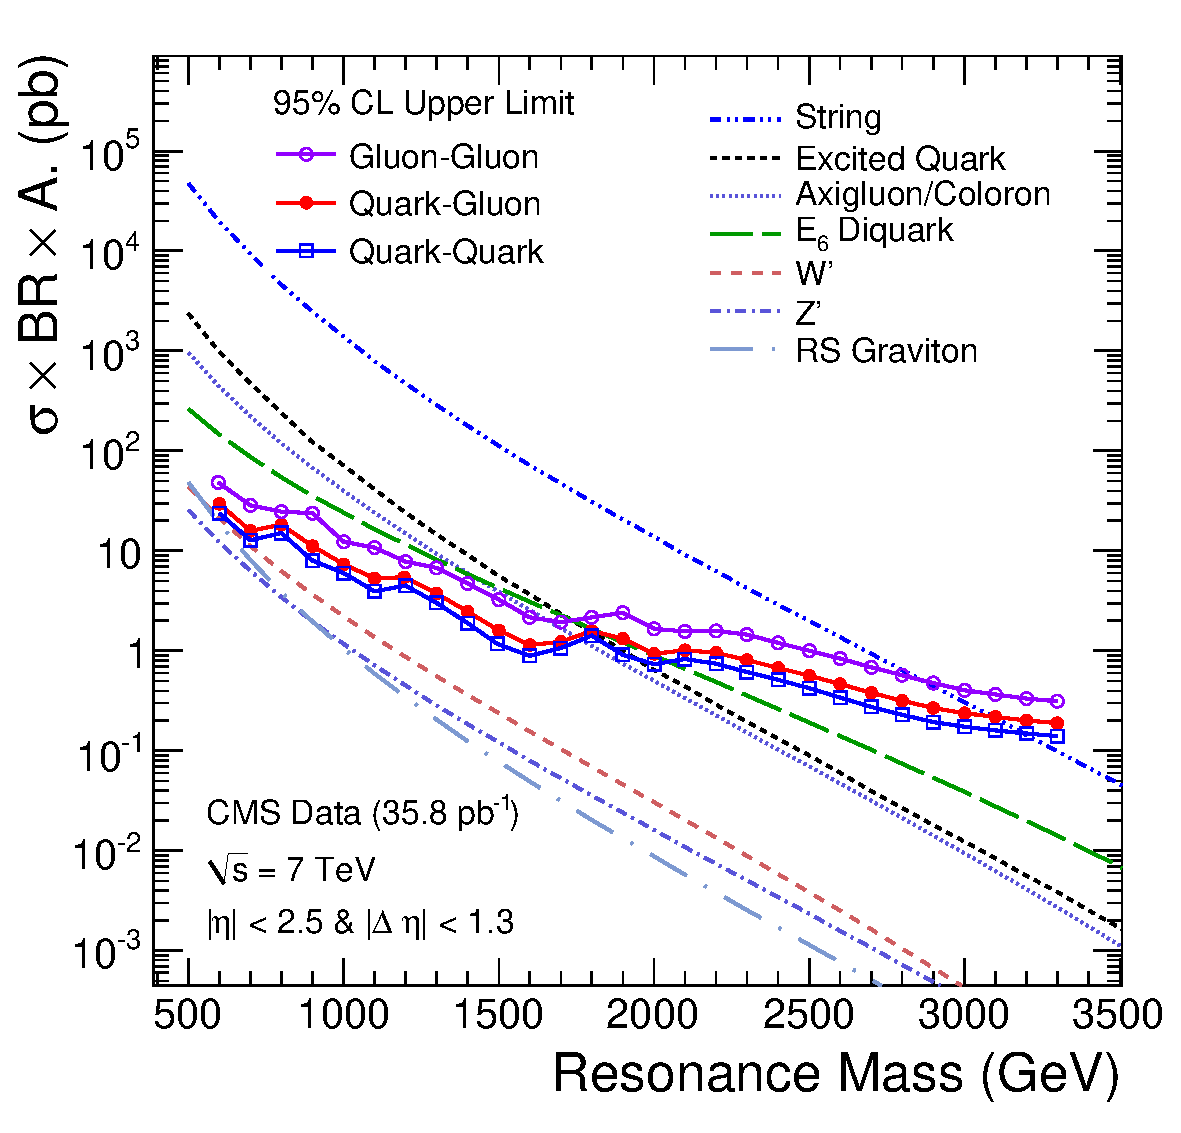
\includegraphics[width=\textwidth]{Figures/Limit_Comp_final.pdf}
%    \caption{ The 95\% CL upper limits on the cross section for 
%    dijet resonances (points) shown seperately for the three different 
%    parton pairs $qq$, $qg$ and $gg$, is 
%    compared to the model cross section for 7 different models (see text).}
%    \label{limit_sys}
%  \end{center}
%\end{figure}


%\begin{table}[htbH]
%\centering
%\large
%\begin{tabular}{|c|c|c|c|}\hline
%Mass   &  \multicolumn{3}{c|}{95\% C.L. $\sigma\cdot B$ (pb)}\\
% ($TeV$) &  quark-quark      & quark-gluon  & gluon-gluon\\ \hline
%0.6	 &  23.8	 &  29.5	 &  47.8  \\  
%0.7	 &  12.7	 &  15.7	 &  28.4  \\  
%0.8	 &  15.1	 &  18.2	 &  24.6  \\  
%0.9	 &  8.01	 &  11.2	 &  23.7  \\  
%1.0	 &  5.99	 &  7.34	 &  12.2  \\  
%1.1	 &  3.93	 &  5.28	 &  10.8  \\  
%1.2	 &  4.47	 &  5.35	 &  7.77  \\  
%1.3	 &  3.04	 &  3.75	 &  6.73  \\  
%1.4	 &  1.89	 &  2.46	 &  4.70  \\  
%1.5	 &  1.14	 &  1.59	 &  3.24  \\  
%1.6	 &  0.89	 &  1.14	 &  2.16  \\  
%1.7	 &  1.06	 &  1.23	 &  1.93  \\  
%1.8	 &  1.41	 &  1.59	 &  2.15  \\  
%1.9	 &  0.910	 &  1.32	 &  2.41  \\  
%2.0	 &  0.729	 &  0.933	 &  1.65  \\  
%2.1	 &  0.831	 &  1.02	 &  1.57  \\  
%2.2	 &  0.741	 &  0.958	 &  1.59  \\  
%2.3	 &  0.611	 &  0.811	 &  1.44  \\  
%2.4	 &  0.511	 &  0.676	 &  1.19  \\  
%2.5	 &  0.424	 &  0.562	 &  1.00  \\  
%2.6	 &  0.341	 &  0.463	 &  0.832 \\  
%2.7	 &  0.274	 &  0.378	 &  0.684 \\  
%2.8	 &  0.228	 &  0.316	 &  0.568 \\  
%2.9	 &  0.194	 &  0.268	 &  0.478 \\  
%3.0	 &  0.174	 &  0.237	 &  0.402 \\  
%3.1	 &  0.160	 &  0.217	 &  0.364 \\  
%3.2	 &  0.149	 &  0.201	 &  0.332 \\  
%3.3	 &  0.140	 &  0.189	 &  0.314 \\
%\hline
%\end{tabular}
%\caption{As a function of resonance mass we list our 95\% C.L. upper limit on
%cross section times branching ratio for narrow resonances originating from   
%quark-quark, quark-gluon, and gluon-gluon pairs of partons,
%including systematic uncertainties.}
%\label{tabXsecLimit}
%\end{table}

\begin{figure}[!ht]
  \begin{center}
    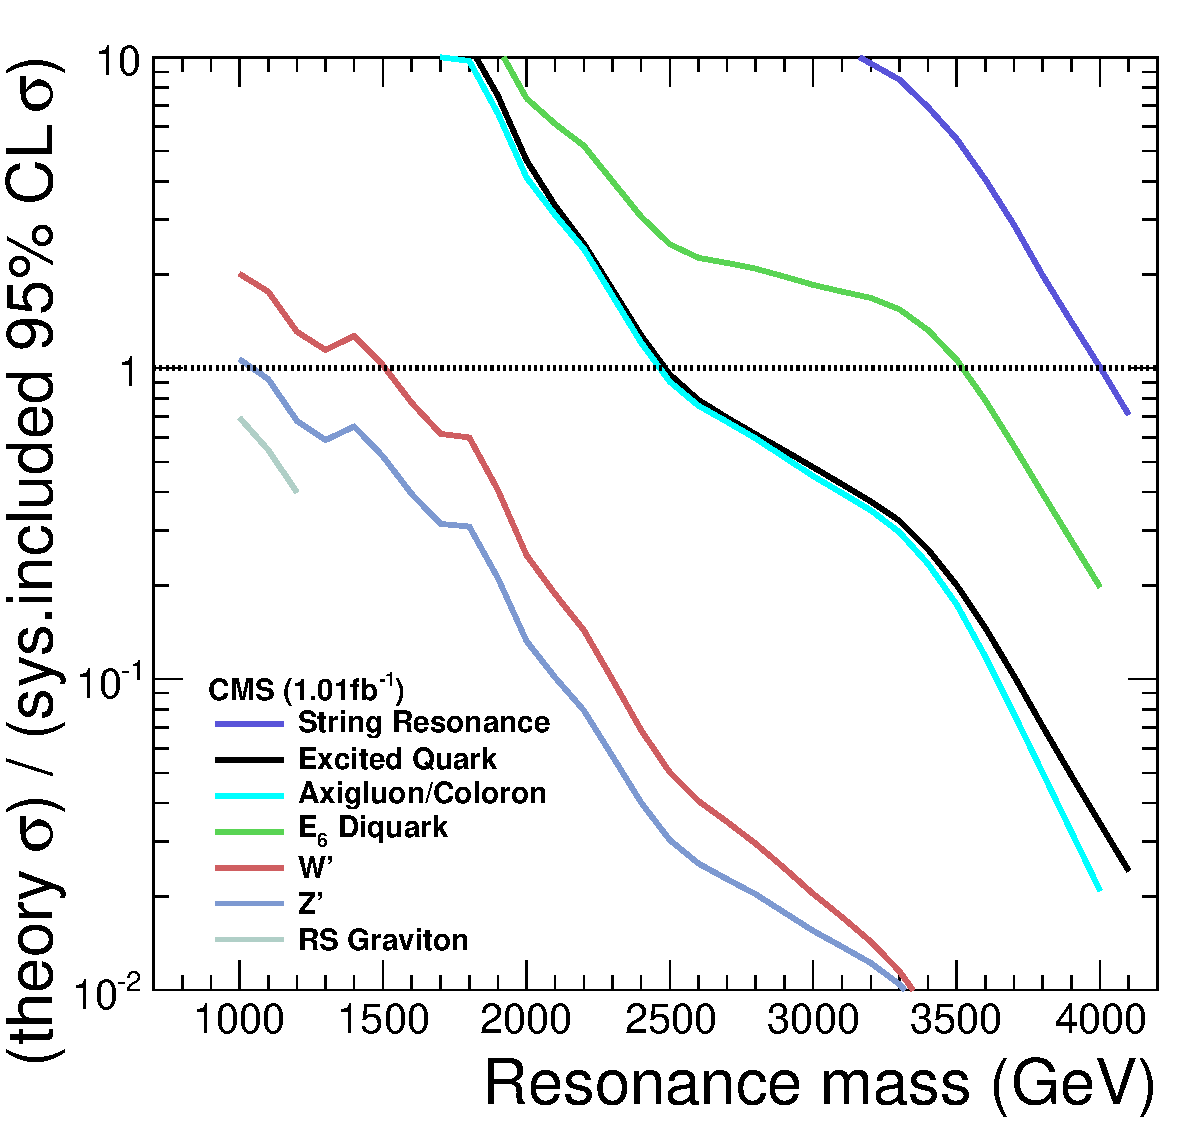
\includegraphics[width=\textwidth]{Figures/c_xs_comparison_bw_sys_theory_fat.pdf}
    \caption{ The model cross section divided by the 95\% CL exclusion upper limits of fat jet result 
      on the cross section for the appropritate parton pairs.}
    \label{limit_ratio_fat}
  \end{center}
\end{figure}

\begin{figure}[!ht]
  \begin{center}
    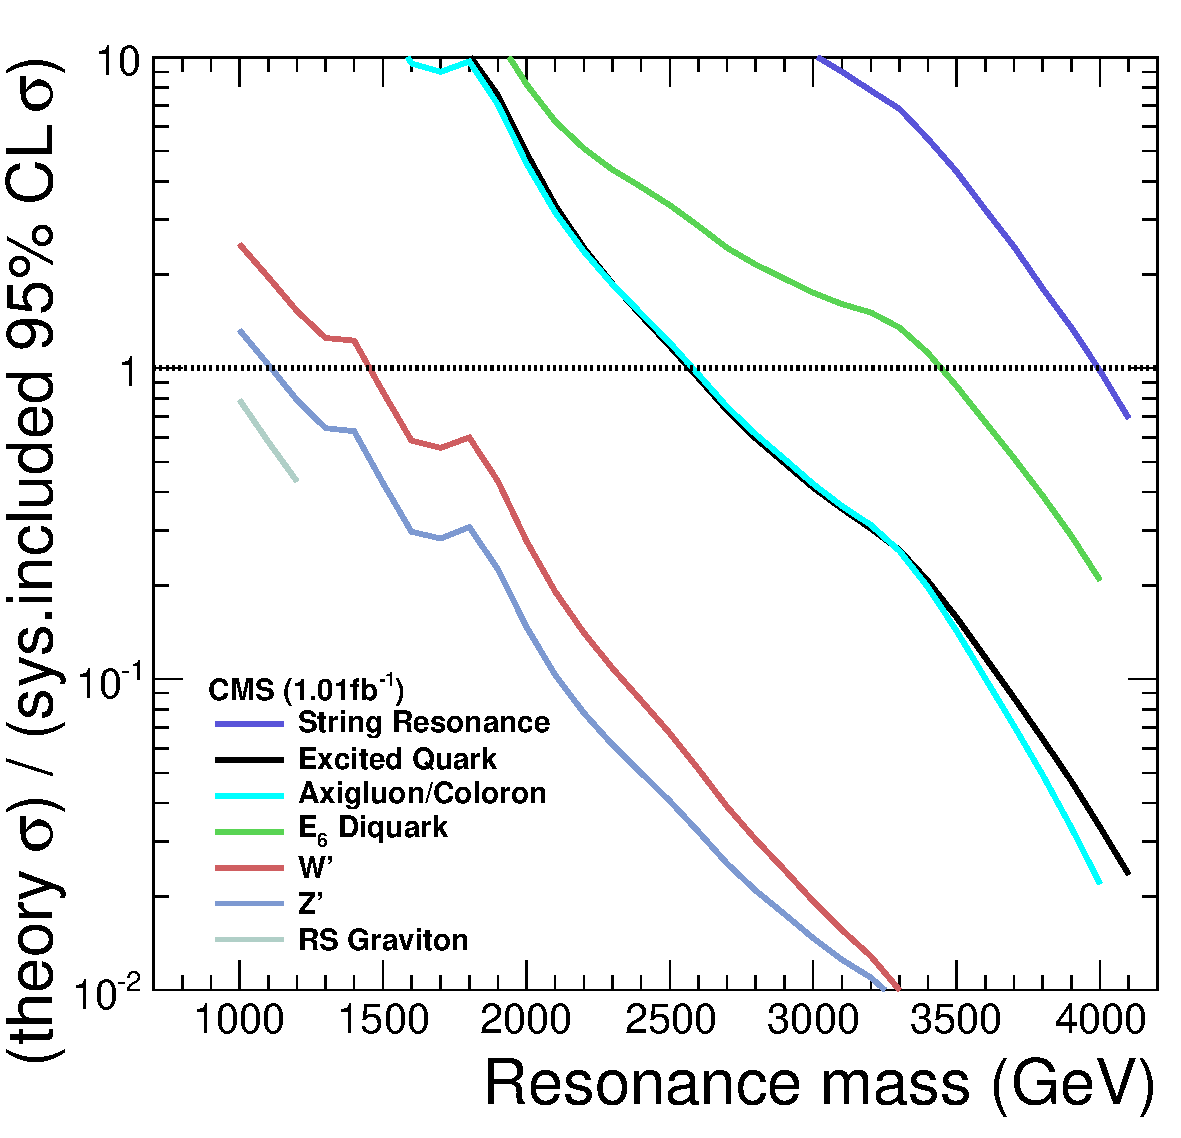
\includegraphics[width=\textwidth]{Figures/c_xs_comparison_bw_sys_theory_pf.pdf}
    \caption{ The model cross section divided by the 95\% CL exclusion upper limits of pf jet result 
      on the cross section for the appropritate parton pairs.}
    \label{limit_ratio_pf}
  \end{center}
\end{figure}

\begin{figure}[!ht]
  \begin{center}
    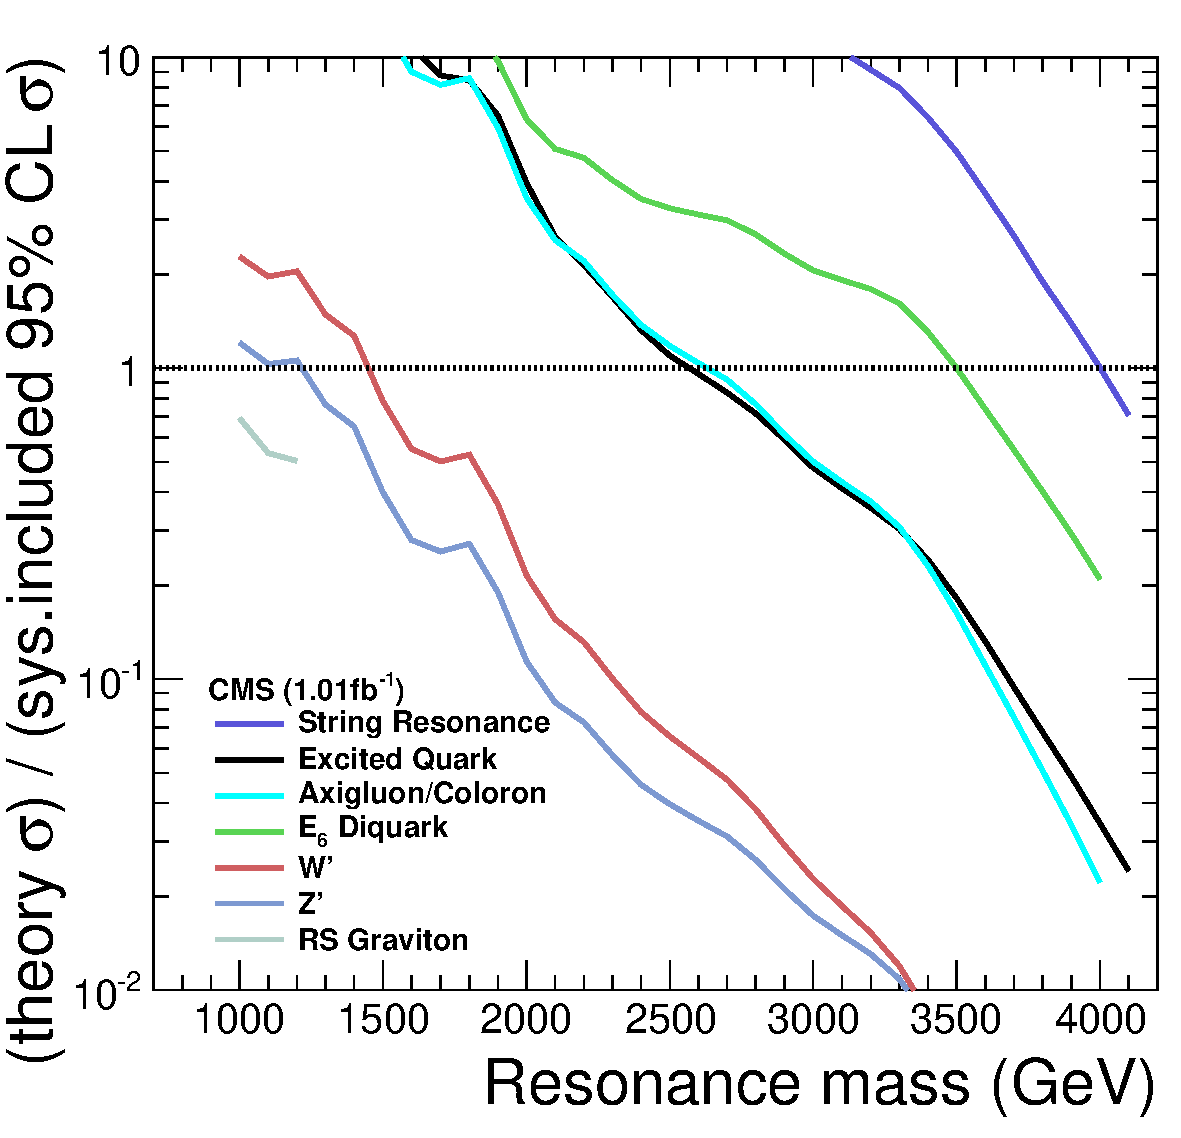
\includegraphics[width=\textwidth]{Figures/c_xs_comparison_bw_sys_theory_calo.pdf}
    \caption{ The model cross section divided by the 95\% CL exclusion upper limits of calo jet result
      on the cross section for the appropritate parton pairs.}
    \label{limit_ratio_calo}
  \end{center}
\end{figure}

\clearpage
